\section{SSIS Toolbox}

\paragraph{Data Flow Task}
Used to move data between sources and destinations. Allows to perform data cleaning and transformations.

\vspace{10pt}
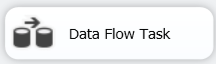
\includegraphics{img/dataflowtask.png}


\paragraph{Execute SQL Task}
Used to execute SQL queries. Can be combined with Data Flow Task to perform ETL operations. Queries can be specified in the editor, under the SQLStatement property.

\vspace{10pt}
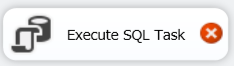
\includegraphics{img/executesqltask.png}

\paragraph{OLE DB Source}
Connects and reads data from and OLE DB database. This component allows the user to choose which table and which columns to read.

\vspace{10pt}
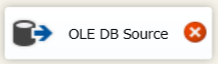
\includegraphics{img/oledbsource.png}

\paragraph{OLE DB Destination}
Connects and writes data to an OLE DB database. This component allows the user to choose which table to write to, as well as the mapping between the input columns and the destination columns.

\vspace{10pt}
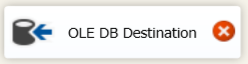
\includegraphics{img/oledbdestination.png}

\paragraph{Flat File Source}
Reads data from flat files (e.g., csv, txt). The user can specify the file path, and which columns/rows to read.

\vspace{10pt}
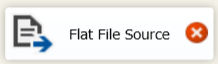
\includegraphics{img/flatfilesource.png}

\paragraph{Flat File Destination}
Writes data to flat files (e.g., csv, txt). The user can specify the file path, and which columns/rows to write.

\vspace{10pt}
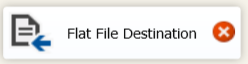
\includegraphics{img/flatfiledestination.png}

\paragraph{Aggregate}
Groups input rows based on the specified columns and aggregates data using a set of available functions (e.g., sum, average, count), depending on the data type.

\vspace{10pt}
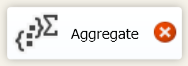
\includegraphics{img/aggregate.png}

\paragraph{Derived Column}
Creates new columns or replaces existing ones with calculated expressions. The editor provides a set of functions and operators to build expressions.

\vspace{10pt}
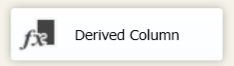
\includegraphics{img/derivedcolumn.png}

\paragraph{Conditional Split}
Splits the data flow into multiple paths based on specified conditions. It behaves like a switch/case statement, and allows a default output for rows that do not match any condition.

\vspace{10pt}

\includegraphics{img/conditionalsplit.png}

\paragraph{Multicast}
Multiplies the input data and sends it to different outputs.

\vspace{10pt}
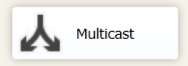
\includegraphics{img/multicast.png}

\paragraph{Sort}
Sorts the input data based on the specified columns and order (ascending/descending). Also allows to remove duplicate rows.

\vspace{10pt}
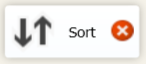
\includegraphics{img/sort.png}

\paragraph{Lookup}
Performs a lookup of input rows against a remote source. It is normally used to add columns to the already available ones. Since it's a lookup, even if a row matches multiples in the source, only the first match is returned. If a row has no match, the editor allows to choose how to handle it (ignore, fail, redirect).

\vspace{10pt}
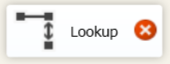
\includegraphics{img/lookup.png}

\paragraph{Union All}
Combines rows from multiple inputs in a single output. It is the equivalent of a SQL UNION ALL operation.

\vspace{10pt}

\includegraphics{img/unionall.png}

\paragraph{Merge}
Similar to Union All, but requires input rows to be sorted, and produces a sorted output.

\vspace{10pt}
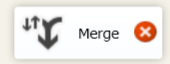
\includegraphics{img/merge.png}

\paragraph{Merge Join}
Implements a join operation (inner, left, full outer), producing only rows that satisfy the join condition. Requires input rows to be sorted.

\vspace{10pt}
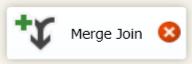
\includegraphics{img/mergejoin.png}

\paragraph{Percentage Sampling}
Randomly selects the specified percentage of rows from the input data.

\vspace{10pt}
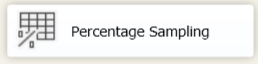
\includegraphics{img/percentagesampling.png}

\paragraph{Row Sampling}
Randomly selects a specified number of rows from the input data.

\vspace{10pt}
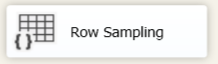
\includegraphics{img/rowsampling.png}